The aim of this chapter is to review

%%%%%%%%%%%%%%%%%%%%%%%%%%%%%%%%%%%%%%%%%%%%%%%%%%%%%%%%%%%%%%%%%%%%
%%%%%%%%%%%%%%%%%%%%%%%%%%%%%%%%%%%%%%%%%%%%%%%%%%%%%%%%%%%%%%%%%%%%
%%%%%%%%%%%%%%%%%%%%%%%%%%%%%%%%%%%%%%%%%%%%%%%%%%%%%%%%%%%%%%%%%%%%

\section{Testing Data}

\subsection{Database Videos}

The system is tested using a database of 50 different videos, ranging from 7 to 14 seconds, as per requirements F25-F26. The database of videos is populated from scratch using free stock footage from \textit{Pexels Video}\footnote{Pexels Video: \url{https://www.pexels.com/videos/}}. The videos used to build the database are chosen from a rich library of videos encapsulating many different colours (e.g. bright, dark, warm, cold, colourful, etc.) and movements (e.g. still, motion, shaky, blurry, timelapses, etc.) to ensure diversification. The database of videos used to test the system can be found in the \textit{``footage''} directory in the provided code.\\

Employing existing databases of videos for CBVR tasks such as the TRECVID\footnote{Text REtrieval Conference Video Retrieval Evaluation} dataset \cite{2018trecvidawad}, which is the best dataset for CBVR-oriented tasks, would have been ideal to measure the project's performance and to compare it with existing solutions for this task. However, these datasets are not publicly available and hard to obtain. For example, most of the referenced papers in the Bibliography that present CBVR solutions were conducted for the TRECVID conferences, meaning that the datasets were provided to the participants for testing and evaluating results. However, the NIST\footnote{National Institute of Standards and Technology, organiser of the annual TRECVID conference} does not provide these databases for external papers. Other databases of videos exist, but target other computer vision tasks such as facial recognition or image retrieval rather than CBVR. Therefore, the previously mentioned custom database of 50 videos is used to test this system.\\

\subsection{Query Videos}

Various query videos are recorded to test the online retrieval phase of the system. These queries are mobile recordings of one of the database videos. Different types of queries listed in Section \ref{sec:design-query-video-processing} are used to test the limits of the system, including down-scaled (recording at a distance from the screen) and skewed queries (recording at an angle) coupled with minor camera movement due to shaking hands. These conditions ensure the realism of the queries if the system were to be developed as a mobile application.

%%%%%%%%%%%%%%%%%%%%%%%%%%%%%%%%%%%%%%%%%%%%%%%%%%%%%%%%%%%%%%%%%%%%
%%%%%%%%%%%%%%%%%%%%%%%%%%%%%%%%%%%%%%%%%%%%%%%%%%%%%%%%%%%%%%%%%%%%
%%%%%%%%%%%%%%%%%%%%%%%%%%%%%%%%%%%%%%%%%%%%%%%%%%%%%%%%%%%%%%%%%%%%

\section{Results Analysis}

\begin{figure}[h] 
\centerline{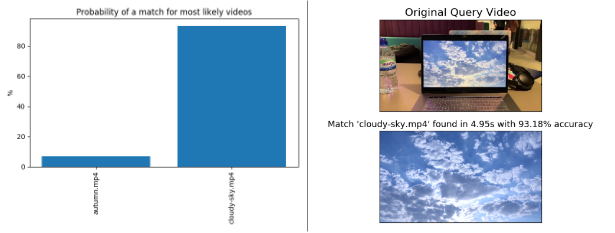
\includegraphics[width=\textwidth]{figures/evaluation/recording1-results.png}}
\caption{\label{fig:design-recording1-results}Recording 1.}
\end{figure}

\begin{figure}[h] 
\centerline{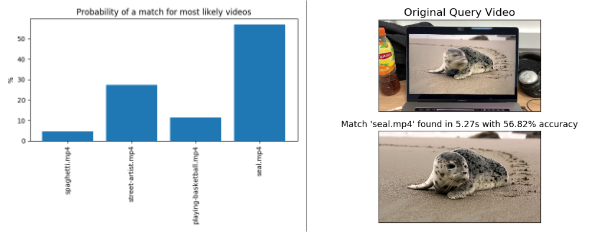
\includegraphics[width=\textwidth]{figures/evaluation/recording2-results.png}}
\caption{\label{fig:design-recording2-results}Recording 2.}
\end{figure}

\begin{figure}[h] 
\centerline{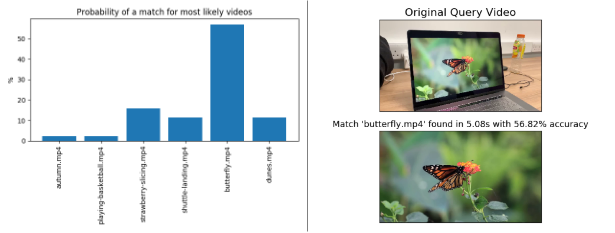
\includegraphics[width=\textwidth]{figures/evaluation/recording3-results.png}}
\caption{\label{fig:design-recording3-results}Recording 3.}
\end{figure}

\subsection{Video Matching}

show quantitative values for different queries:
    \begin{itemize}
        \item number of True Positives 
        \item number of False Positives
        \item general accuracy
    \end{itemize}

runtime

\subsection{Movie Segmentation}

The shot boundary detection algorithm is used on a feature-length movie. The movie used for the test is Inception\footnote{Inception IMDb page: https://www.imdb.com/title/tt1375666/}. The movie is composed of 213098 frames.

The shot boundary detection algorithm is used once with the KL Divergence and once with the Intersection metric..

\begin{itemize}
    \item KL Divergence: a global threshold of 10 using the KL Divergence detects 661 shot boundaries (0,31\%) in 149.7 minutes.
    \item Intersection: A global threshold of 7 using the Intersection metric detects 1730 shot boundaries (0.81\%).
\end{itemize}

\begin{figure}[h] 
\centerline{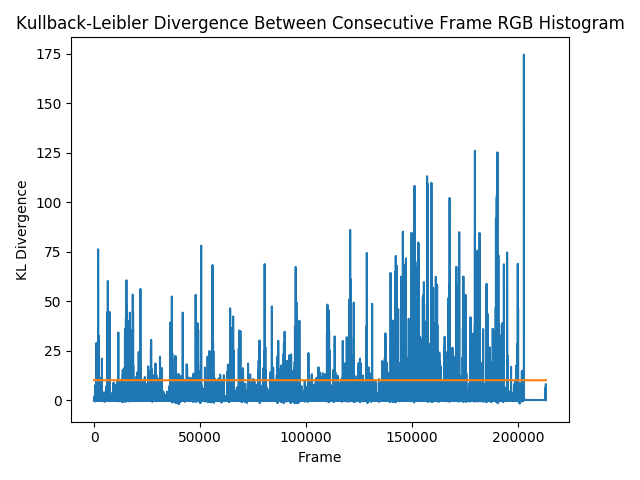
\includegraphics[width=0.70\textwidth]{figures/evaluation/inception_KLdiv_threshold10.png}}
\caption{\label{fig:inception_KLdiv_threshold10}Result of the shot boundary detection algorithm on the Inception movie using the KL Divergence between consecutive frames' RGB histograms.}
\end{figure}

\begin{figure}[h] 
\centerline{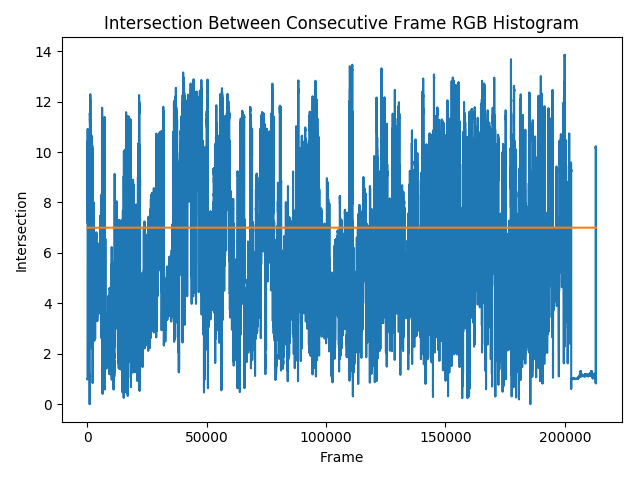
\includegraphics[width=0.70\textwidth]{figures/evaluation/inception_inter_threshold7.png}}
\caption{\label{fig:inception_inter_threshold7}Result of the shot boundary detection algorithm on the Inception movie using the Intersection between consecutive frames' RGB histograms.}
\end{figure}

%%%%%%%%%%%%%%%%%%%%%%%%%%%%%%%%%%%%%%%%%%%%%%%%%%%%%%%%%%%%%%%%%%%%
%%%%%%%%%%%%%%%%%%%%%%%%%%%%%%%%%%%%%%%%%%%%%%%%%%%%%%%%%%%%%%%%%%%%
%%%%%%%%%%%%%%%%%%%%%%%%%%%%%%%%%%%%%%%%%%%%%%%%%%%%%%%%%%%%%%%%%%%%

\section{Individual Models and Metrics Analysis}

analyse results of RGB, grey scale and HSV histograms with the 6 different histogram matching methods. which work best? in which scenarios

removing KL divergence metric greatly improved accuracy. (using less metric to use the ones for the job). KL divergence NEVER found correct match, not meant to be used a distance metric (show example of removing KL div and alternate chi square with past examples and new one)

%%%%%%%%%%%%%%%%%%%%%%%%%%%%%%%%%%%%%%%%%%%%%%%%%%%%%%%%%%%%%%%%%%%%
%%%%%%%%%%%%%%%%%%%%%%%%%%%%%%%%%%%%%%%%%%%%%%%%%%%%%%%%%%%%%%%%%%%%
%%%%%%%%%%%%%%%%%%%%%%%%%%%%%%%%%%%%%%%%%%%%%%%%%%%%%%%%%%%%%%%%%%%%

\section{Observations}

general observation: lighting affecting system accuracy (at night time, in dark room with small lamps that produce yellow light)

%%%%%%%%%%%%%%%%%%%%%%%%%%%%%%%%%%%%%%%%%%%%%%%%%%%%%%%%%%%%%%%%%%%%
%%%%%%%%%%%%%%%%%%%%%%%%%%%%%%%%%%%%%%%%%%%%%%%%%%%%%%%%%%%%%%%%%%%%
%%%%%%%%%%%%%%%%%%%%%%%%%%%%%%%%%%%%%%%%%%%%%%%%%%%%%%%%%%%%%%%%%%%%

\section{Comparison With Ground Truth Experiment}

online classification experiment:
    \begin{itemize}
        \item Google Survey experiment results 
        \item Compare experiment results with the algorithm results
        \item use a plot to visualise experiment results
        \item link to appendix (Ethics Checklist Appendix \ref{ch:appendix-ethics-checklist}, Experiment Script Appendix \ref{ch:appendix-experiment-survey}, and Raw Results)
    \end{itemize}
    
mention ground truth (https://en.wikipedia.org/wiki/Ground\_truth) (https://www.techopedia.com/definition/32514/ground-truth)

%%%%%%%%%%%%%%%%%%%%%%%%%%%%%%%%%%%%%%%%%%%%%%%%%%%%%%%%%%%%%%%%%%%%
%%%%%%%%%%%%%%%%%%%%%%%%%%%%%%%%%%%%%%%%%%%%%%%%%%%%%%%%%%%%%%%%%%%%
%%%%%%%%%%%%%%%%%%%%%%%%%%%%%%%%%%%%%%%%%%%%%%%%%%%%%%%%%%%%%%%%%%%%

\section{Summary}

todo